%%%%%%%%%%%%%%%%%%%%%%%%%%%%%%%%%%%%%%%%%
% Short Sectioned Assignment LaTeX Template Version 1.0 (5/5/12)
% This template has been downloaded from: http://www.LaTeXTemplates.com
% Original author:  Frits Wenneker (http://www.howtotex.com)
% License: CC BY-NC-SA 3.0 (http://creativecommons.org/licenses/by-nc-sa/3.0/)
%%%%%%%%%%%%%%%%%%%%%%%%%%%%%%%%%%%%%%%%%

%----------------------------------------------------------------------------------------
%	PACKAGES AND OTHER DOCUMENT CONFIGURATIONS
%----------------------------------------------------------------------------------------

\documentclass[paper=a4, fontsize=11pt]{scrartcl} % A4 paper and 11pt font size

% ---- Entrada y salida de texto -----

\usepackage[T1]{fontenc} % Use 8-bit encoding that has 256 glyphs
\usepackage[utf8]{inputenc}
%\usepackage{fourier} % Use the Adobe Utopia font for the document - comment this line to return to the LaTeX default

% ---- Idioma --------

\usepackage[spanish, es-tabla]{babel} % Selecciona el español para palabras introducidas automáticamente, p.ej. "septiembre" en la fecha y especifica que se use la palabra Tabla en vez de Cuadro

% ---- Otros paquetes ----

\usepackage{url} % ,href} %para incluir URLs e hipervínculos dentro del texto (aunque hay que instalar href)
\usepackage{amsmath,amsfonts,amsthm} % Math packages
%\usepackage{graphics,graphicx, floatrow} %para incluir imágenes y notas en las imágenes
\usepackage{graphics,graphicx, float} %para incluir imágenes y colocarlas

% Para hacer tablas comlejas
%\usepackage{multirow}
%\usepackage{threeparttable}

%\usepackage{sectsty} % Allows customizing section commands
%\allsectionsfont{\centering \normalfont\scshape} % Make all sections centered, the default font and small caps

\usepackage{fancyhdr} % Custom headers and footers
\pagestyle{fancyplain} % Makes all pages in the document conform to the custom headers and footers
\fancyhead{} % No page header - if you want one, create it in the same way as the footers below
\fancyfoot[L]{} % Empty left footer
\fancyfoot[C]{} % Empty center footer
\fancyfoot[R]{\thepage} % Page numbering for right footer
\renewcommand{\headrulewidth}{0pt} % Remove header underlines
\renewcommand{\footrulewidth}{0pt} % Remove footer underlines
\setlength{\headheight}{13.6pt} % Customize the height of the header

\numberwithin{equation}{section} % Number equations within sections (i.e. 1.1, 1.2, 2.1, 2.2 instead of 1, 2, 3, 4)
\numberwithin{figure}{section} % Number figures within sections (i.e. 1.1, 1.2, 2.1, 2.2 instead of 1, 2, 3, 4)
\numberwithin{table}{section} % Number tables within sections (i.e. 1.1, 1.2, 2.1, 2.2 instead of 1, 2, 3, 4)

\setlength\parindent{0pt} % Removes all indentation from paragraphs - comment this line for an assignment with lots of text

\newcommand{\horrule}[1]{\rule{\linewidth}{#1}} % Create horizontal rule command with 1 argument of height

%\documentclass{report}
\usepackage{blindtext}
\usepackage{hyperref}
\usepackage{listings}
\usepackage{graphicx}
\graphicspath{ {images/} }

\title{	
\normalfont \normalsize 
\textsc{\textbf{Ingeniería de Servidores (2022-2023)} \\ Grado en Ingeniería Informática \\ Universidad de Granada} \\ [25pt] % Your university, school and/or department name(s)
\horrule{0.5pt} \\[0.4cm] % Thin top horizontal rule
\huge Memoria Práctica 3 \\ % The assignment title
\horrule{2pt} \\[0.5cm] % Thick bottom horizontal rule
}

\author{Francisco Javier Gallardo Molina} % Nombre y apellidos

\date{\normalsize\today} % Incluye la fecha actual

\renewcommand{\footrulewidth}{0.4pt}
\lfoot[]{Francisco Javier Gallardo Molina}
\rfoot[]{\thepage}

\begin{document}

\maketitle

\newpage

\horrule{1pt}
\tableofcontents

\newpage

\section{Instalación de máquinas virtuales}

Para la realización de esta práctica, debemos de hacer una instalación de dos máquinas virtuales, una que haga de servidor y una de cliente. Para la máquina servidor se usará Ubuntu 20.04 y para el cliente Rocky Linux 9.0. Para cada máquina debemos tener un sistema de archivos RAID1 instalado, por lo que debemos tener la siguiente configuración en Ubuntu como se ve en la figura \ref{fig:lsblk-ubuntu}.\\

\begin{figure}[H]
  \centering
  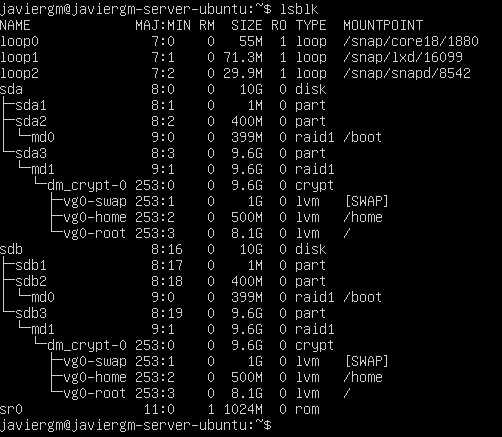
\includegraphics[scale=0.9]{Captura1}
  \caption{Sistema de archivos RAID1 en Ubuntu}
  \label{fig:lsblk-ubuntu}
\end{figure}

De igual manera, Rocky debe de tener una configuración similar a esta figura \ref{fig:lsblk-rocky}.\\

\begin{figure}[H]
  \centering
  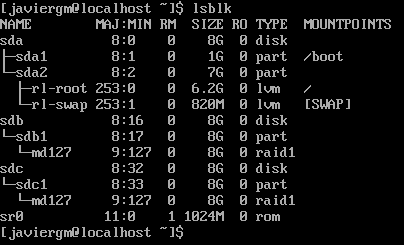
\includegraphics[scale=0.9]{Captura2}
  \caption{Sistema de archivos RAID1 en Rocky Linux}
  \label{fig:lsblk-rocky}
\end{figure}

\section{Zabbix}

\subsection{Instalación y configuración del servidor en Ubuntu 20}
Para la instalación de Zabbix en la máquina virtual he seguido este manual 
\url{https://www.zabbix.com/download?zabbix=5.0&os_distribution=ubuntu&os_version=20.04_focal&db=mysql&ws=apache} para instalar el servidor y el agente de Zabbix.\\

Lo primero que hay que hacer es instalar el repositorio de Zabbix en la máquina usando los siguientes comandos:

\begin{lstlisting}
> wget  https://repo.zabbix.com/zabbix/5.0/ubuntu/pool/main/z/
zabbix-release/zabbix-release_5.0-1+focal_all.deb
\end{lstlisting}

\begin{lstlisting}
> sudo dpkg -i zabbix-release_5.0-1+focal_all.deb
\end{lstlisting}

\begin{lstlisting}
> sudo apt update
\end{lstlisting}

Tras instalar el repositorio, en lugar de usar un proxy para la instalación he preferido seguir con este manual \url{https://www.zabbix.com/download?zabbix=5.0&os_distribution=debian&os_version=10_buster&db=mysql} y usar los paquetes de zabbix de frontend, servidor y agente:

\begin{lstlisting}
> sudo apt install zabbix-server-mysql zabbix-frontend-php 
zabbix-apache-conf zabbix-agent 
\end{lstlisting}

Con todo ya instalado, procedemos a configurar la base de datos con la que Zabbix va a trabajar. Para ello, primero tenemos que instalar la base de datos, que en mi caso será MySQL:

\begin{lstlisting}
> sudo apt install mysql-server
\end{lstlisting}

Una vez instalada, debemos crear la base de datos que el servidor usará. Para ello debemos de entrar en el prompt de MySQL con el siguiente comando:

\begin{lstlisting}
> sudo mysql -u root -p
\end{lstlisting}

Cabe destacar que tras ejecutar este comando nos pedirá contraseña, pero al no haber hecho una configuración previa, no habrá que introducir nada y nos permitirá entrar en el prompt de la base de datos sin problemas. Dentro de este prompt, realizamos la configuración que se indica en la documentación de Zabbix o en la figura \ref{fig:mysql}.

\begin{figure}[H]
  \centering
  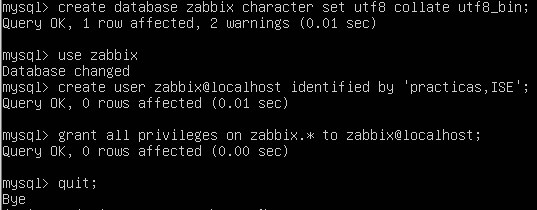
\includegraphics{Captura3}
  \caption{Configuración de la base de datos de Zabbix}
  \label{fig:mysql}
\end{figure}

Una vez creada la base de datos, seguimos la documentación de Zabbix y ejecutamos el siguiente comando:\\

\begin{lstlisting}
> zcat /usr/share/doc/zabbix-server-mysql*/create.sql.gz | mysql
-uzabbix -p zabbix
\end{lstlisting}

Nos pedirá una contraseña y debemos de meter la que se ha indicado en la \ref{fig:mysql}, que en mi caso es \textit{practicas,ISE}. Después de esto, saltó un error de los discos bastante grande \ref{fig:error}.

\begin{figure}[H]
  \centering
  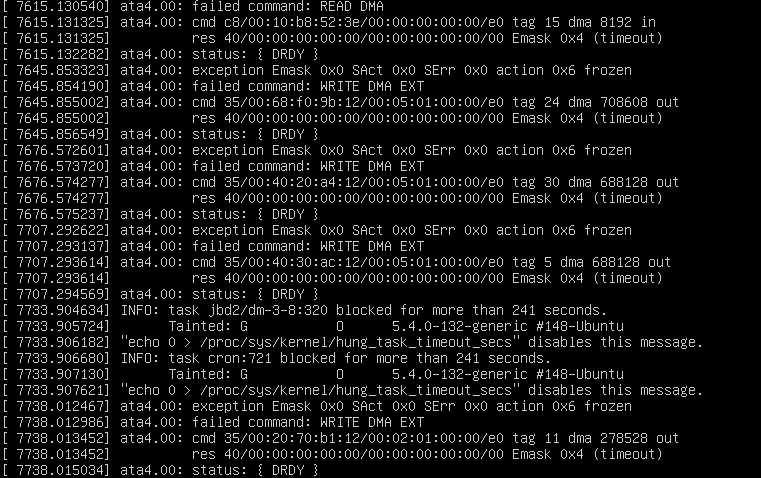
\includegraphics[scale=0.9]{error}
  \caption{Error mostrado}
  \label{fig:error}
\end{figure}

Puesto que no me dejó realizar ninguna acción, tuve que matar el proceso de VirtualBox para poder apagar la máquina. Tras eso, encendí de nuevo la máquina esperando que se hubiera roto todo, pero sorprendentemente, no hubo problemas al iniciar. Probé a introducir el comando de nuevo, pero me mostró por pantalla que los datos estaban ya creados, así que aparentemente todo estaba normal,  por lo que decidí continuar con la instalación.\\

Con todo esto hecho, pasamos a modificar los archivos de configuración de Zabbix para indicarle cuál es la contraseña que hemos introducido. Para ello nos vamos al archivo '/etc/zabbix/zabbix\_server.conf' y modificamos la sección en la que pone 'DBPassword', descomentamos la instrucción y ponemos nuestra contraseña como se indica en la figura \ref{fig:zabbix-conf}.

\begin{figure}[H]
  \centering
  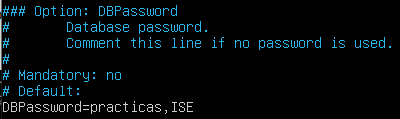
\includegraphics{Captura4}
  \caption{Contraseña de Zabbix en archivo de configuración}
  \label{fig:zabbix-conf}
\end{figure}

Por último modificamos el archivo '/etc/zabbix/apache.conf' para cambiar el huso horario de nuestro servidor de Zabbix como se indica la figura \ref{fig:zabbix-conf-apache}:

\begin{figure}[H]
  \centering
  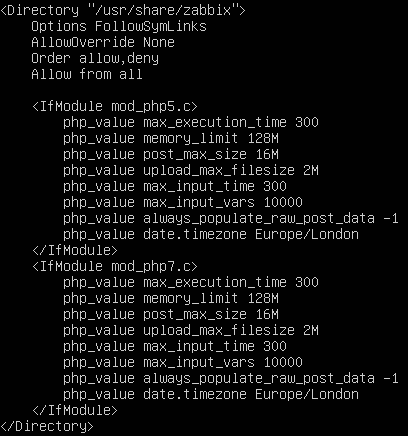
\includegraphics[scale=0.9]{Captura5}
  \caption{Huso horario de Zabbix}
  \label{fig:zabbix-conf-apache}
\end{figure}

Con todo esto hecho, reiniciamos el servidor de Zabbix junto con su agente y apache2:

\begin{lstlisting}
> sudo systemctl restart zabbix-server zabbix-agent apache2
\end{lstlisting}

\begin{lstlisting}
> sudo systemctl enable zabbix-server zabbix-agent apache2 
\end{lstlisting}

Tras esto, comprobamos que los servicios de MySQL, Apache2 y Zabbix estén funcionando, como aparece en las figuras \ref{fig:estado-mysql}, \ref{fig:estado-apache} y \ref{fig:estado-zabbix}.


\begin{figure}[H]
  \centering
  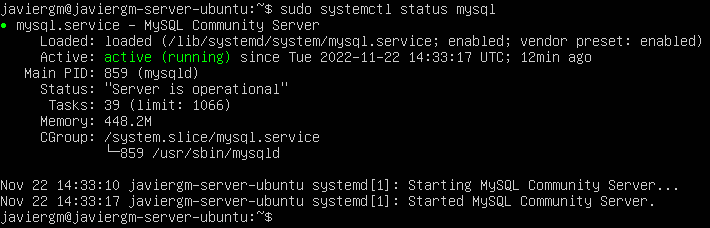
\includegraphics[scale=0.9]{Captura6}
  \caption{Estado del servicio de MySQL}
  \label{fig:estado-mysql}
\end{figure}

\begin{figure}[H]
  \centering
  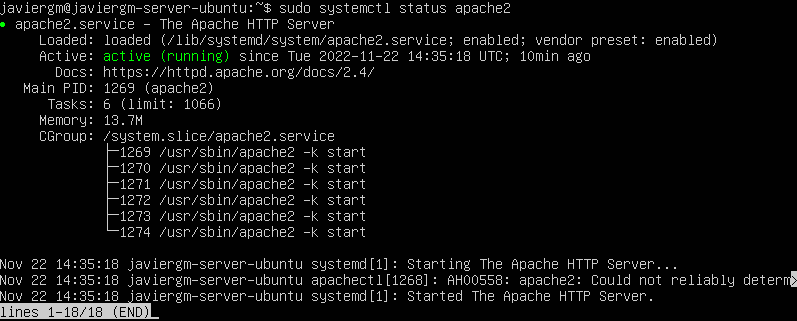
\includegraphics[scale=0.9]{Captura7}
  \caption{Estado del servicio de Apache2}
  \label{fig:estado-apache}
\end{figure}

\begin{figure}[H]
  \centering
  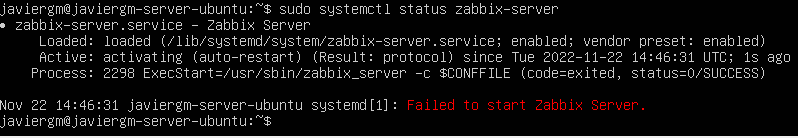
\includegraphics[scale=0.9]{Captura8}
  \caption{Estado del servicio de Zabbix-server}
  \label{fig:estado-zabbix}
\end{figure}

Al comprobar el estado de Zabbix, vemos que ha fallado al iniciar el servicio. Este error tras investigar junto con la ayuda del profesor, vimos que se debía a un fallo al importar los datos a la base de datos y que está relacionado con el error \ref{fig:error}. Para solucionarlo, tuvimos que borrar la base de datos de Zabbix y volverla a crear, pero al tratar de crear los datos del usuario de Zabbix, nos mostraba por pantalla que no se podía. Al final la solución fue realizar esta serie de comandos:

\begin{lstlisting}
mysql> drop user zabbix@localhost; 
\end{lstlisting}

\begin{lstlisting}
mysql> flush privileges;
\end{lstlisting}

\begin{lstlisting}
mysql> create user zabbix@localhost identified by 'practicas,ISE'
\end{lstlisting}

\begin{lstlisting}
mysql> grant all privileges on zabbix.* to zabbix@localhost;
\end{lstlisting}

Una vez hecho esto, volvimos a importar los datos de Zabbix con el comando:

\begin{lstlisting}
> zcat /usr/share/doc/zabbix-server-mysql*/create.sql.gz | mysql
-uzabbix -p zabbix
\end{lstlisting}

Nos volvió a pedir la contraseña, y tras introducirla, se copiaron los datos sin que saltara el error \ref{fig:error}. Puesto que parece estar todo correcto, probamos a comprobar el estado del servicio de Zabbix-server \ref{fig:estado-zabbix-correcto}.

\begin{figure}[H]
  \centering
  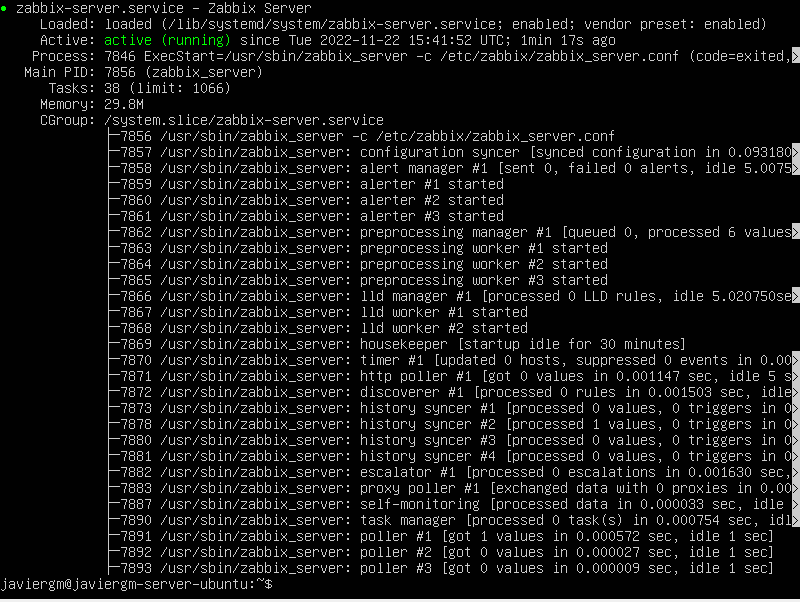
\includegraphics[scale=0.7]{Captura9}
  \caption{Estado del servicio de Zabbix-server}
  \label{fig:estado-zabbix-correcto}
\end{figure}

Puesto que ya funciona, la configuración del servidor está terminada.\\

Como parte opcional, para hacer la instalación de la base de datos de MySQL más segura, es recomendable usar el comando de "mysql\_secure\_installation" para ajustar ciertos parámetros como establecer una contraseña para la cuenta de root o desactivar el acceso remoto al usuario root.\\

Si bien con todo esto ya podríamos usar el servidor de Zabbix para monitorizar el servidor puede ser que no podamos acceder a Zabbix desde el navegador, como ocurrió en mi caso. Puede ser debido a que la interfaz de red no tenga asignada una IP con la que se pueda conectar a la máquina virtual o que no tenga el adaptador de red solo-anfitrión activado. Para que funcione, debemos de activar otro adaptador de red en VirtualBox que sea solo-anfitrión como indica la figura \ref{fig:adaptador}.\\

\begin{figure}[H]
  \centering
  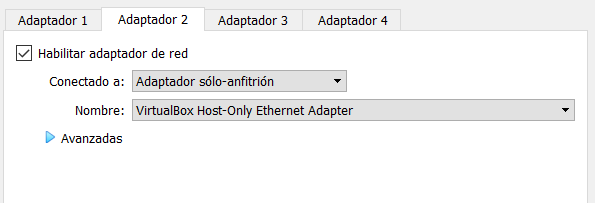
\includegraphics{Captura10}
  \caption{Adaptador solo-anfitrión}
  \label{fig:adaptador}
\end{figure}

Tras esto, ejecutamos 'ip addr' para comprobar su ip, pero vemos que no aparece nada. Debemos de asociarle una ip y activar la interfaz con los siguientes comandos:

\begin{lstlisting}
> sudo ip addr add 192.168.56.115/24 dev enp0s8
\end{lstlisting}

\begin{lstlisting}
> sudo ip link set enp0s8 up
\end{lstlisting}

\begin{figure}[H]
  \centering
  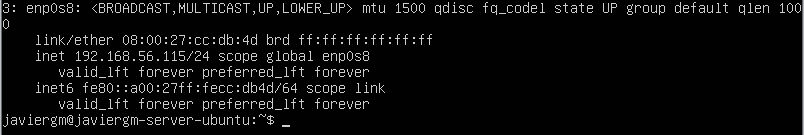
\includegraphics[scale=0.8]{Captura11}
  \caption{IP de la máquina}
  \label{fig:ip}
\end{figure}

Un problema que puede surgir es que el cortafuegos de Windows, como es mi caso, no nos permita conectarnos a Zabbix desde el navegador. Debemos de entrar en la configuración avanzada del cortafuegos y en el apartado de \textit{Reglas de entrada} añadimos una regla que permita la conexión de nuestro PC con la máquina virtual a través de las IPs.\\

Realizado todo el proceso de la IP, ya podemos proceder a instalar y configurar el frontend de Zabbix. Es un proceso rápido por lo que no tiene mucha complicación. Debemos de indicar la base de datos de Zabbix y su contraseña \ref{fig:conf-frontend}. El resto de configuración lo dejamos por defecto.

\begin{figure}[H]
  \centering
  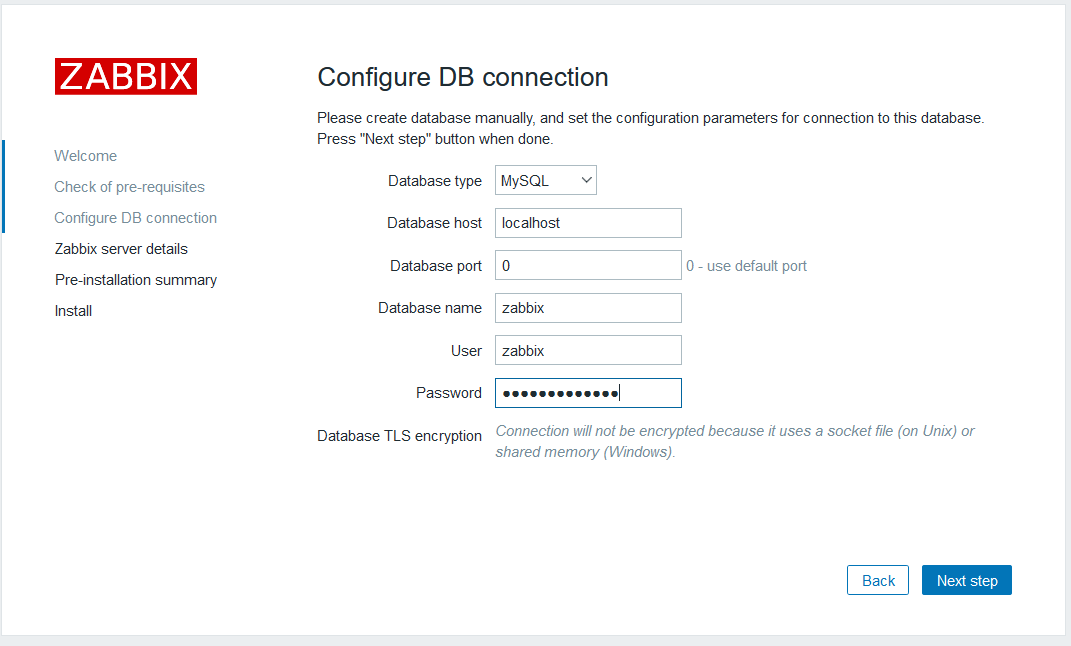
\includegraphics[scale=0.6]{Captura12}
  \caption{Configuración de Zabbix en navegador}
  \label{fig:conf-frontend}
\end{figure}

Por úlitmo, nos pedirá que iniciemos sesión y usaremos el usuario por defecto \textit{Admin} y la contraseña \textit{zabbix}. Iniciando sesión, ya tendremos listo nuestro servidor para monitorizar.
